% Options for packages loaded elsewhere
\PassOptionsToPackage{unicode}{hyperref}
\PassOptionsToPackage{hyphens}{url}
%
\documentclass[
]{article}
\usepackage{lmodern}
\usepackage{amssymb,amsmath}
\usepackage{ifxetex,ifluatex}
\ifnum 0\ifxetex 1\fi\ifluatex 1\fi=0 % if pdftex
  \usepackage[T1]{fontenc}
  \usepackage[utf8]{inputenc}
  \usepackage{textcomp} % provide euro and other symbols
\else % if luatex or xetex
  \usepackage{unicode-math}
  \defaultfontfeatures{Scale=MatchLowercase}
  \defaultfontfeatures[\rmfamily]{Ligatures=TeX,Scale=1}
\fi
% Use upquote if available, for straight quotes in verbatim environments
\IfFileExists{upquote.sty}{\usepackage{upquote}}{}
\IfFileExists{microtype.sty}{% use microtype if available
  \usepackage[]{microtype}
  \UseMicrotypeSet[protrusion]{basicmath} % disable protrusion for tt fonts
}{}
\makeatletter
\@ifundefined{KOMAClassName}{% if non-KOMA class
  \IfFileExists{parskip.sty}{%
    \usepackage{parskip}
  }{% else
    \setlength{\parindent}{0pt}
    \setlength{\parskip}{6pt plus 2pt minus 1pt}}
}{% if KOMA class
  \KOMAoptions{parskip=half}}
\makeatother
\usepackage{xcolor}
\IfFileExists{xurl.sty}{\usepackage{xurl}}{} % add URL line breaks if available
\IfFileExists{bookmark.sty}{\usepackage{bookmark}}{\usepackage{hyperref}}
\hypersetup{
  pdftitle={Shelton et al.~2021 SI Appendix},
  hidelinks,
  pdfcreator={LaTeX via pandoc}}
\urlstyle{same} % disable monospaced font for URLs
\usepackage[margin=1in]{geometry}
\usepackage{longtable,booktabs}
% Correct order of tables after \paragraph or \subparagraph
\usepackage{etoolbox}
\makeatletter
\patchcmd\longtable{\par}{\if@noskipsec\mbox{}\fi\par}{}{}
\makeatother
% Allow footnotes in longtable head/foot
\IfFileExists{footnotehyper.sty}{\usepackage{footnotehyper}}{\usepackage{footnote}}
\makesavenoteenv{longtable}
\usepackage{graphicx,grffile}
\makeatletter
\def\maxwidth{\ifdim\Gin@nat@width>\linewidth\linewidth\else\Gin@nat@width\fi}
\def\maxheight{\ifdim\Gin@nat@height>\textheight\textheight\else\Gin@nat@height\fi}
\makeatother
% Scale images if necessary, so that they will not overflow the page
% margins by default, and it is still possible to overwrite the defaults
% using explicit options in \includegraphics[width, height, ...]{}
\setkeys{Gin}{width=\maxwidth,height=\maxheight,keepaspectratio}
% Set default figure placement to htbp
\makeatletter
\def\fps@figure{htbp}
\makeatother
\setlength{\emergencystretch}{3em} % prevent overfull lines
\providecommand{\tightlist}{%
  \setlength{\itemsep}{0pt}\setlength{\parskip}{0pt}}
\setcounter{secnumdepth}{-\maxdimen} % remove section numbering

\title{Shelton et al.~2021 SI Appendix}
\author{}
\date{\vspace{-2.5em}}

\begin{document}
\maketitle

{
\setcounter{tocdepth}{2}
\tableofcontents
}
\renewcommand{\thefigure}{S\arabic{figure}}
\setcounter{figure}{0}

\renewcommand{\thetable}{S\arabic{table}}
\setcounter{table}{0}

\clearpage

\hypertarget{environmental-dna-laboratory-analysis-details-and-diagnostics}{%
\section{Environmental DNA laboratory analysis details and
diagnostics}\label{environmental-dna-laboratory-analysis-details-and-diagnostics}}

This section provides detailed information about the analysis of eDNA
collected during the 2019 US-Canada Integrated Ecosystem and Pacific
Hake Acoustic-Trawl Survey (1). The statistical model for eDNA is
presented in the main text.

\hypertarget{standards}{%
\subsubsection{Standards}\label{standards}}

For each qPCR plate, we included samples with a known number of hake DNA
copies to allow us to translate the observed PCR cycle at which
amplification occurred to the number of copies in a sample. We present
both the relationship for the PCR cycle at which amplification was
observed (Fig. \ref{fig:stand}) and the probability of observing
amplification at different DNA copy numbers (Fig. \ref{fig:stand.pres}).
We followed (2) for creating standard curves but with threee additional
replicates at 5 \(copies\) \(\mu L^{-1}\) and six replicates at 1
\(copies\) \(\mu L^{-1}\). The analysis of standards shows that our qPCR
analyses were sensitive to very low copy numbers and consistent across
plates.

\begin{figure}
\includegraphics[width=1\linewidth]{Supplement_S1_files/figure-latex/fig.stand-1} \caption{\label{fig:stand} qPCR standards for 33 plates with DNA copy numbers ranging from 1 to 100,000.}\label{fig:fig.stand}
\end{figure}

\begin{figure}
\includegraphics[width=0.75\linewidth]{Supplement_S1_files/figure-latex/fig.stand.pres-1} \caption{\label{fig:stand.pres} Amplification success for qPCR standards for 33 plates with DNA copy numbers ranging from 1 to 100,000.}\label{fig:fig.stand.pres}
\end{figure}

\hypertarget{investigations-of-contamination.}{%
\subsubsection{Investigations of
contamination.}\label{investigations-of-contamination.}}

In addition to field samples, we collected control samples ship board to
look for potential contamination of samples during sample processing. We
collected 2 L of distilled water from either the onboard evaporator or
from distilled water brought from the laboratory for this purpose
(\(N=49\)). We found low levels of contamination in both types of
control samples and lump them together for further analysis. While 18 of
49 had hake DNA below the detection limit of 20 \(copies L^{-1}\), 31
had higher concentrations. Of these 31 samples, most (21 samples) had
very low concentrations \(<100\) \(copies L^{-1}\) but there was a
single sample with \(>500\) \(copies L^{-1}\) (Fig.
\ref{fig:contam.hist}). From these observations, we estimated the
parameters from a log-normal distribution to describe the distribution
of hake DNA from contamination (Fig. \ref{fig:contam.hist}; posterior
mean estimates: \(\mu\) = 3.5, \(\sigma =\) 0.767).This corresponds to
an expected contribution of 44.4 copies per liter per sample. For this
distribution 92\% of samples would be expected to have less than 100
\emph{copies} \(L^{-1}\) but there will be a small number of more
significantly contaminated samples. We remain unsure of the ultimate
source of contamination in these samples but are conducting additional
sampling during the survey cruise of 2021 to identify and eliminate
contamination.

Numerous negative controls PCR were included in each qPCR plate and
these controls showed no amplification.

To understand the potential effect of contamination on our results, we
first plotted the estimated distribution from contamination against the
estimates of hake DNA concentration in field samples (Fig.
\ref{fig:contam.facet}). The observed hake DNA distributions were all
substantially larger than estimated contamination distribution. So while
contamination may be playing a minor role in determining the observed
hake DNA, it is not a dominant factor determining the spatial or depth
specific distribution of DNA. We cannot identify which samples have a
significant contribution of contamination but there is no suggestion
that the contamination has a spatial or depth-specific effect. Such
contamination will have a minor effect on the overall DNA abundance,
producing a slight upward bias in the eDNA index. However, as such
contamination is a uniform offset among all samples, it will have no
broad-scale effect on the correlations between eDNA and acoustic-trawl
results in 2019.

\begin{figure}
\includegraphics[width=0.8\linewidth]{Supplement_S1_files/figure-latex/fig.contam.hist-1} \caption{\label{fig:contam.hist} Histogram of point estimates for hake DNA \emph{copies} \(L^{-1}\) from the two types of field control samples (N=49).  Blue line shows estimated lognormal distribution from the observed hake DNA \emph{copies} \(L^{-1}\).}\label{fig:fig.contam.hist}
\end{figure}

\begin{figure}
\includegraphics[width=1\linewidth,height=1\textheight]{Supplement_S1_files/figure-latex/fig.contam.facet-1} \caption{\label{fig:contam.facet} Empirical histograms of estimated hake DNA \emph{copies} \(L^{-1}\) for individual samples at six water depths (purple) and estimated distribution of contamination derived from control samples. Vertical dashed line shows 20 \emph{copies} \(L^{-1}\), the putative detection threshold for our methodology. Note that the x-axis is on the \(log_{10}\) scale.}\label{fig:fig.contam.facet}
\end{figure}

\hypertarget{inhibition}{%
\subsubsection{Inhibition}\label{inhibition}}

As part of our qPCR protocol (2), we included an internal positive
control (IPC) of the reaction to account for PCR inhibition. Any delay
of more than 0.5 cycles from the IPC at the non-template controls of the
PCR was considered inhibition. Inhibited samples were initially purified
using an inhibitor removal column and thereafter diluted 1:2, 1:5 and
1:10 to circumvent inhibition and requantified. We detected inhibition
primarily in the near-surface samples (Fig. \ref{fig:inhibition.depth}).
After inspection of qPCR results following dilution, we included only
1:5 dilution samples in the final statistical model.

\begin{figure}
\includegraphics[width=0.9\linewidth,height=0.9\textheight]{Supplement_S1_files/figure-latex/fig.inhibition.depth -1} \caption{\label{fig:inhibition.depth} Samples that were identified as being inhibited by sample depths.  Samples identified as being inhibited were diluted and re-run using quantitative PCR. }\label{fig:fig.inhibition.depth }
\end{figure}

\hypertarget{ethanol-wash-error}{%
\subsubsection{Ethanol wash error}\label{ethanol-wash-error}}

For a subset of samples, DNA extraction was incorrectly washed with
overdiluted ethanol at the final desalting step of the DNA purification.
Specifically, samples were washed with a 30\% ethanol solution instead
of a 70\% ethanol solution. Affected samples lost of some DNA during the
washing processes. Washed bottles were geographically restricted to the
northern part of the sample area, but occurred across all sample depths
(Fig. \ref{fig:wash.plot}). To examine the magnitude of this problem, we
experimentally divided samples taken from 26 individual station-depth
combinations and subjected one bottle taken from those stations to the
proper 70\% ethanol wash and for the paired bottle used a 30\% ethanol
wash. This paired design allowed us to estimate the magnitude of the DNA
concentration lost due to the wash error.

Within the model we estimate that this washing error led to
\(\omega =\)-0.56 {[}-0.7, -0.41{]} (mean {[}95\% CI{]}), which
traslates to approximately 72.27\% of the DNA being lost due to the
ethanol wash error (Fig. \ref{fig:wash.hist}).

\begin{figure}
\includegraphics[width=0.75\linewidth]{Supplement_S1_files/figure-latex/fig.wash.plot -1} \caption{\label{fig:wash.plot} Samples that were identified using the overdiluted ethanol wash. Samples identified as being diluted were included in the statistical model.}\label{fig:fig.wash.plot }
\end{figure}

\begin{figure}
\includegraphics[width=0.6\linewidth]{Supplement_S1_files/figure-latex/fig.wash.hist -1} \caption{\label{fig:wash.hist} Posterior estimate of \(\omega\), the offset due to the ethanol was error. Vertical dashed line indicates posterior mean. }\label{fig:fig.wash.hist }
\end{figure}

\newpage
\clearpage

\hypertarget{edna-model-fit-diagnostics-and-supplementary-figures}{%
\section{eDNA model: fit, diagnostics, and supplementary
figures}\label{edna-model-fit-diagnostics-and-supplementary-figures}}

During prelimiary model fits, we investigated a range of knot densities
used to describe smooth terms. To balance computational speed and model
flexibility, we settled on using 5 knots for the bottom depth smooth and
a 4 (longitudinal axis) by 10 (latitudinal axis) knot grid for the
tensor-smoothes. Model results are largely insensitive to knot density.

Prior distributions for all parameters are presented in Table S1.1. We
utilize the package \emph{brms} to generate design matrices necessary to
estimate smooth terms. Thus we use the random effect representation of
smoothes to estimate the model as a generalized linear mixed model. This
is equivalent to using the \(t2()\) function in the commonly used
\emph{mgcv} package for GAMs. This represents the non-linear components
of the spline basis as random effects and their associated variance
parameters control the wiggliness of the estimated splines (3, 4).

\begin{longtable}[]{@{}ll@{}}
\caption{Prior and parameter descriptions for the eDNA
Model.}\tabularnewline
\toprule
\begin{minipage}[b]{0.47\columnwidth}\raggedright
Parameter \& Prior\strut
\end{minipage} & \begin{minipage}[b]{0.47\columnwidth}\raggedright
Description\strut
\end{minipage}\tabularnewline
\midrule
\endfirsthead
\toprule
\begin{minipage}[b]{0.47\columnwidth}\raggedright
Parameter \& Prior\strut
\end{minipage} & \begin{minipage}[b]{0.47\columnwidth}\raggedright
Description\strut
\end{minipage}\tabularnewline
\midrule
\endhead
\begin{minipage}[t]{0.47\columnwidth}\raggedright
Process Model Components (\(D_{xyd}\))\strut
\end{minipage} & \begin{minipage}[t]{0.47\columnwidth}\raggedright
\strut
\end{minipage}\tabularnewline
\begin{minipage}[t]{0.47\columnwidth}\raggedright
\(\gamma_d \sim Normal(0,5)\)\strut
\end{minipage} & \begin{minipage}[t]{0.47\columnwidth}\raggedright
Spatial intercept for DNA concentration at each depth \(d\)\strut
\end{minipage}\tabularnewline
\begin{minipage}[t]{0.47\columnwidth}\raggedright
\(b_s \sim Normal(0,5)\)\strut
\end{minipage} & \begin{minipage}[t]{0.47\columnwidth}\raggedright
Linear component for each spline and tensor smooth\strut
\end{minipage}\tabularnewline
\begin{minipage}[t]{0.47\columnwidth}\raggedright
\(s_k \sim Normal(0,\xi_k)\)\strut
\end{minipage} & \begin{minipage}[t]{0.47\columnwidth}\raggedright
Value for spline knot \(k\)\strut
\end{minipage}\tabularnewline
\begin{minipage}[t]{0.47\columnwidth}\raggedright
\(\xi_k \sim T(3,0,2.5)\)\strut
\end{minipage} & \begin{minipage}[t]{0.47\columnwidth}\raggedright
Standard deviation for spline knot \(k\)\strut
\end{minipage}\tabularnewline
\begin{minipage}[t]{0.47\columnwidth}\raggedright
\strut
\end{minipage} & \begin{minipage}[t]{0.47\columnwidth}\raggedright
\strut
\end{minipage}\tabularnewline
\begin{minipage}[t]{0.47\columnwidth}\raggedright
Observation Model Components\strut
\end{minipage} & \begin{minipage}[t]{0.47\columnwidth}\raggedright
\strut
\end{minipage}\tabularnewline
\begin{minipage}[t]{0.47\columnwidth}\raggedright
\(\tau \sim Normal(0,2)\)\strut
\end{minipage} & \begin{minipage}[t]{0.47\columnwidth}\raggedright
Standard deviation for among Niskin bottle\strut
\end{minipage}\tabularnewline
\begin{minipage}[t]{0.47\columnwidth}\raggedright
\(\omega \sim Normal(-1,1)\)\strut
\end{minipage} & \begin{minipage}[t]{0.47\columnwidth}\raggedright
Ethanol wash offset\strut
\end{minipage}\tabularnewline
\begin{minipage}[t]{0.47\columnwidth}\raggedright
\(\phi_0 \sim Normal(2,2)\)\strut
\end{minipage} & \begin{minipage}[t]{0.47\columnwidth}\raggedright
PCR amplification detection intercept\strut
\end{minipage}\tabularnewline
\begin{minipage}[t]{0.47\columnwidth}\raggedright
\(\phi_1 \sim Normal(4,2)\)\strut
\end{minipage} & \begin{minipage}[t]{0.47\columnwidth}\raggedright
PCR amplification detection slope\strut
\end{minipage}\tabularnewline
\begin{minipage}[t]{0.47\columnwidth}\raggedright
\(\nu = 3\)\strut
\end{minipage} & \begin{minipage}[t]{0.47\columnwidth}\raggedright
T-distribution degrees of freedom (fixed)\strut
\end{minipage}\tabularnewline
\begin{minipage}[t]{0.47\columnwidth}\raggedright
\(\beta_0 \sim Normal(38,4)\)\strut
\end{minipage} & \begin{minipage}[t]{0.47\columnwidth}\raggedright
PCR amplification standards intercept\strut
\end{minipage}\tabularnewline
\begin{minipage}[t]{0.47\columnwidth}\raggedright
\(\beta_1 \sim Normal(-3.22,0.1)\)\strut
\end{minipage} & \begin{minipage}[t]{0.47\columnwidth}\raggedright
PCR amplification standards slope\strut
\end{minipage}\tabularnewline
\begin{minipage}[t]{0.47\columnwidth}\raggedright
\(\sigma \sim Half-Normal(0,2)\)\strut
\end{minipage} & \begin{minipage}[t]{0.47\columnwidth}\raggedright
PCR amplification standards standard deviation\strut
\end{minipage}\tabularnewline
\begin{minipage}[t]{0.47\columnwidth}\raggedright
\(\eta \sim Half-Normal(0,2)\)\strut
\end{minipage} & \begin{minipage}[t]{0.47\columnwidth}\raggedright
PCR amplification field samples scale parameter\strut
\end{minipage}\tabularnewline
\bottomrule
\end{longtable}

\hypertarget{measures-of-fit-and-uncertainty}{%
\subsubsection{Measures of fit and
uncertainty}\label{measures-of-fit-and-uncertainty}}

It is important to illustrate uncertainty bounds for results from the
eDNA model. We capture the mean predictions in the main text (Fig. 1).
Here we present the coefficient of variation (SD / Mean) for hake DNA
concentration (Fig. \ref{fig:cv.maps}). The CV for each predicted
location is derived from 4000 MCMC samples from the joint posterior. CVs
are dramatically larger at shallow depths (3m and 50m). There are two
major drivers of the this pattern in uncertainty for the eDNA model. The
first is that the small scale differences between samples is much larger
at shallow depths than at deep depths. This can be seen clearly in Fig.
\ref{fig:bottle.var.depth} which shows the standard deviation among
samples from a single depth-station by the water depth (\(\tau_d\)).
Recall the the units of \(\tau_d\) are \(log_{10}\) DNA \(copies\)
\(L^{-1}\) so a change from the point estimate of 0.52 at 500m to 0.85
at 3m is substantial. In addition to larger between bottle variability
at shallow depths, there was also a prevalence of large DNA
concentrations in near-surface samples.

These observations were poorly predicted by our statistical model as
evidenced in plots showing the predicted DNA concentration at each
location against the estimated DNA concentration in individual Niskin
bottles (Fig. \ref{fig:pred.obs.edna}). Note that the scatter around the
one-to-one line decreases with increased depth. These very large
observations do not follow an obvious spatial pattern, either (Fig.
\ref{fig:red.delta}). We note that the 3m samples were collected through
the ship's water intake as opposed to the Niskin bottles used at deeper
depths, but we do not know why this would cause the observed patterns.

Overall, the model is able to make reasonable predictions that match
well the observed detection of PCR amplification (Fig.
\ref{fig:pred.obs.edna.raw1}) and, if amplification was detected, the
PCR cycle at which amplification occured (Fig.
\ref{fig:pred.obs.edna.raw2}). While there is a clear, tight
relationship between the observed and predicted values, there is an
increase in scatter for larger PCR cycles (larger observed PCR cycle at
amplification correspond to lower DNA concentrations; see also Fig.
\ref{fig:stand}). This indicates that there is some decrease in fit at
large PCR cycles (low DNA concentrations). While the relationship
between PCR amplification cycle and DNA concentration varies by PCR
reaction (Fig. \ref{fig:stand}), averaged across all PCR plates, an
amplification cycle of \(\sim 36.2\) indicates an approximate DNA
concentration of 40 \(copies\) \(L^{-1}\) and an amplification cycle of
\(\sim 39.5\) is associated with a concentration of 4 \(copies\)
\(L^{-1}\). This means that the lack of fit at large PCR cycles suggests
the model is having difficulty determining the precise DNA concentration
when concentrations are low. High DNA concentrations are well predicted.

\begin{figure}
\includegraphics[width=0.9\linewidth,height=0.9\textheight]{Supplement_S1_files/figure-latex/fig.cv.maps -1} \caption{\label{fig:cv.maps} Posterior estimates of the CV of hake DNA concentration by sampled depth}\label{fig:fig.cv.maps }
\end{figure}

\begin{figure}
\includegraphics[width=0.75\linewidth]{Supplement_S1_files/figure-latex/fig.bottle.var.depth -1} \caption{\label{fig:bottle.var.depth} Estimates of TAU (log10 standard deviation of hake eDNA concentration between bottles at a single station-depth) for each sampling depth (posterior mean and 90 CI shown). Bottles at a sample location become increasingly similar at deeper sampling depths }\label{fig:fig.bottle.var.depth }
\end{figure}

\begin{figure}
\includegraphics[width=0.75\linewidth]{Supplement_S1_files/figure-latex/fig.pred.obs.edna -1} \caption{\label{fig:pred.obs.edna} DNA concentration for each Niskin bottle and sampling site by sample depth. Each point represents the estimated concentration in each Niskin bottle after accounting for multiple PCR replicates.}\label{fig:fig.pred.obs.edna }
\end{figure}

\begin{figure}
\includegraphics[width=1\linewidth,height=1\textheight]{./Pub_Figs/Hake transect DNA D_delta red lat.long.smooth _ Base_Var _ 4_10_fix_nu_T-FIN } \caption{\label{fig:red.delta} Derived estimates of hake DNA concentration at in each Niskin bottle.  Facets show values for each depth category. }\label{fig:fig.red.delta }
\end{figure}

\begin{figure}
\includegraphics[width=0.75\linewidth]{Supplement_S1_files/figure-latex/fig.pred.obs.edna.raw1 -1} \caption{\label{fig:pred.obs.edna.raw1} Predicted probability of PCR amplification from the statistical model plotted against observed amplification (1) or non-amplification (0) for individual samples. Each point represents an individual PCR reaction from a single Niskin bottle.}\label{fig:fig.pred.obs.edna.raw1 }
\end{figure}

\begin{figure}
\includegraphics[width=0.75\linewidth]{Supplement_S1_files/figure-latex/fig.pred.obs.edna.raw2 -1} \caption{\label{fig:pred.obs.edna.raw2} Predicted PCR cycles from the statistical model plotted against observed PCR cycles. Each point represents an individual PCR reaction from a single Niskin bottle. Smaller PCR cycles are associated with higher DNA concentrations while larger PCR cycles are associated with lower DNA concentrations.}\label{fig:fig.pred.obs.edna.raw2 }
\end{figure}

For completeness, we provide estimates of the remaining variance
parameters in the model. The parameter \(\eta\) scales the variability
among PCR replicates for field samples in which a PCR cycle of
amplification was observed (see eq. 5). We estimate \(\eta =\)
0.454{[}0.438,0.472{]} (posterior mean{[}95\% CI{]}). The parameter
\(\sigma\) provides the variability among PCR replicates for known
concentration standards (see eq. 7). We estimate \(\sigma=\)
0.487{[}0.46,0.515{]}.

\hypertarget{estimated-smooth-relationships-for-edna}{%
\subsubsection{Estimated smooth relationships for
eDNA}\label{estimated-smooth-relationships-for-edna}}

We include a smooth for bottom depth in the model for eDNA. It was
estimated to be strongly positive in shallow depths before declining and
becoming more uncertain (Fig. \ref{fig:depth.smooth.edna}). Note that
this covariate is shared among all sampled water depths. To compare with
the smooth for the acoustic-trawl results, see Fig.
\ref{fig:depth.smooth.AT}.

\begin{figure}
\includegraphics[width=0.75\linewidth]{Supplement_S1_files/figure-latex/fig.depth.smooth.edna -1} \caption{\label{fig:depth.smooth.edna} Estimated marignal smooth from the spatial eDNA model.  Units are \(log_{10}\) DNA \emph{copies} \(L^{-1}\).  Posterior mean and 95\% CI shown.}\label{fig:fig.depth.smooth.edna }
\end{figure}

\hypertarget{comparison-of-edna-and-acoustics-trawl-with-alternate-spatial-breaks}{%
\subsubsection{Comparison of eDNA and Acoustics-Trawl with alternate
spatial
breaks}\label{comparison-of-edna-and-acoustics-trawl-with-alternate-spatial-breaks}}

To ensure that the relationship between hake age 2+ biomass and the eDNA
index was not a fluke, we compared the corrlelations between biomass and
eDNA using several different ways of dividing up the coast. As an
example, Fig. \ref{fig:surface.compare.half} shows the domain divided
into half-degree latitudinal bins (Fig. 2 in the main text uses one
degree bins) and Fig. \ref{fig:pairwise} provides the corresponding
correlation between eDNA and acoustic-trawl estimated biomass. The
correlation between eDNA and acoustics is quite high (\(\rho =\)
0.78{[}0.51, 0.91{]}) though somewhat lower than the correlation of 0.87
for the one degree bins (see main text).

\begin{figure}
\includegraphics[width=1\linewidth]{./Pub_Figs/Hake_maps_combined_to_surface_half_degree} \caption{\label{fig:surface.compare.half} 2019 survey locations (left; red circles show eDNA sampling locations, lines show acoustic transects), depth-integrated  index of hake DNA (middle) and hake biomass from acoustic surveys (right).  Both DNA and acoustic estimates are mean predicted values projected to a 5km grid and include information between 50 and 500m deep. All panels show half-degree latitudinal bins used to aggregate abundance estimates over larger spatial scales.    }\label{fig:fig.surface.compare.half}
\end{figure}

\begin{figure}
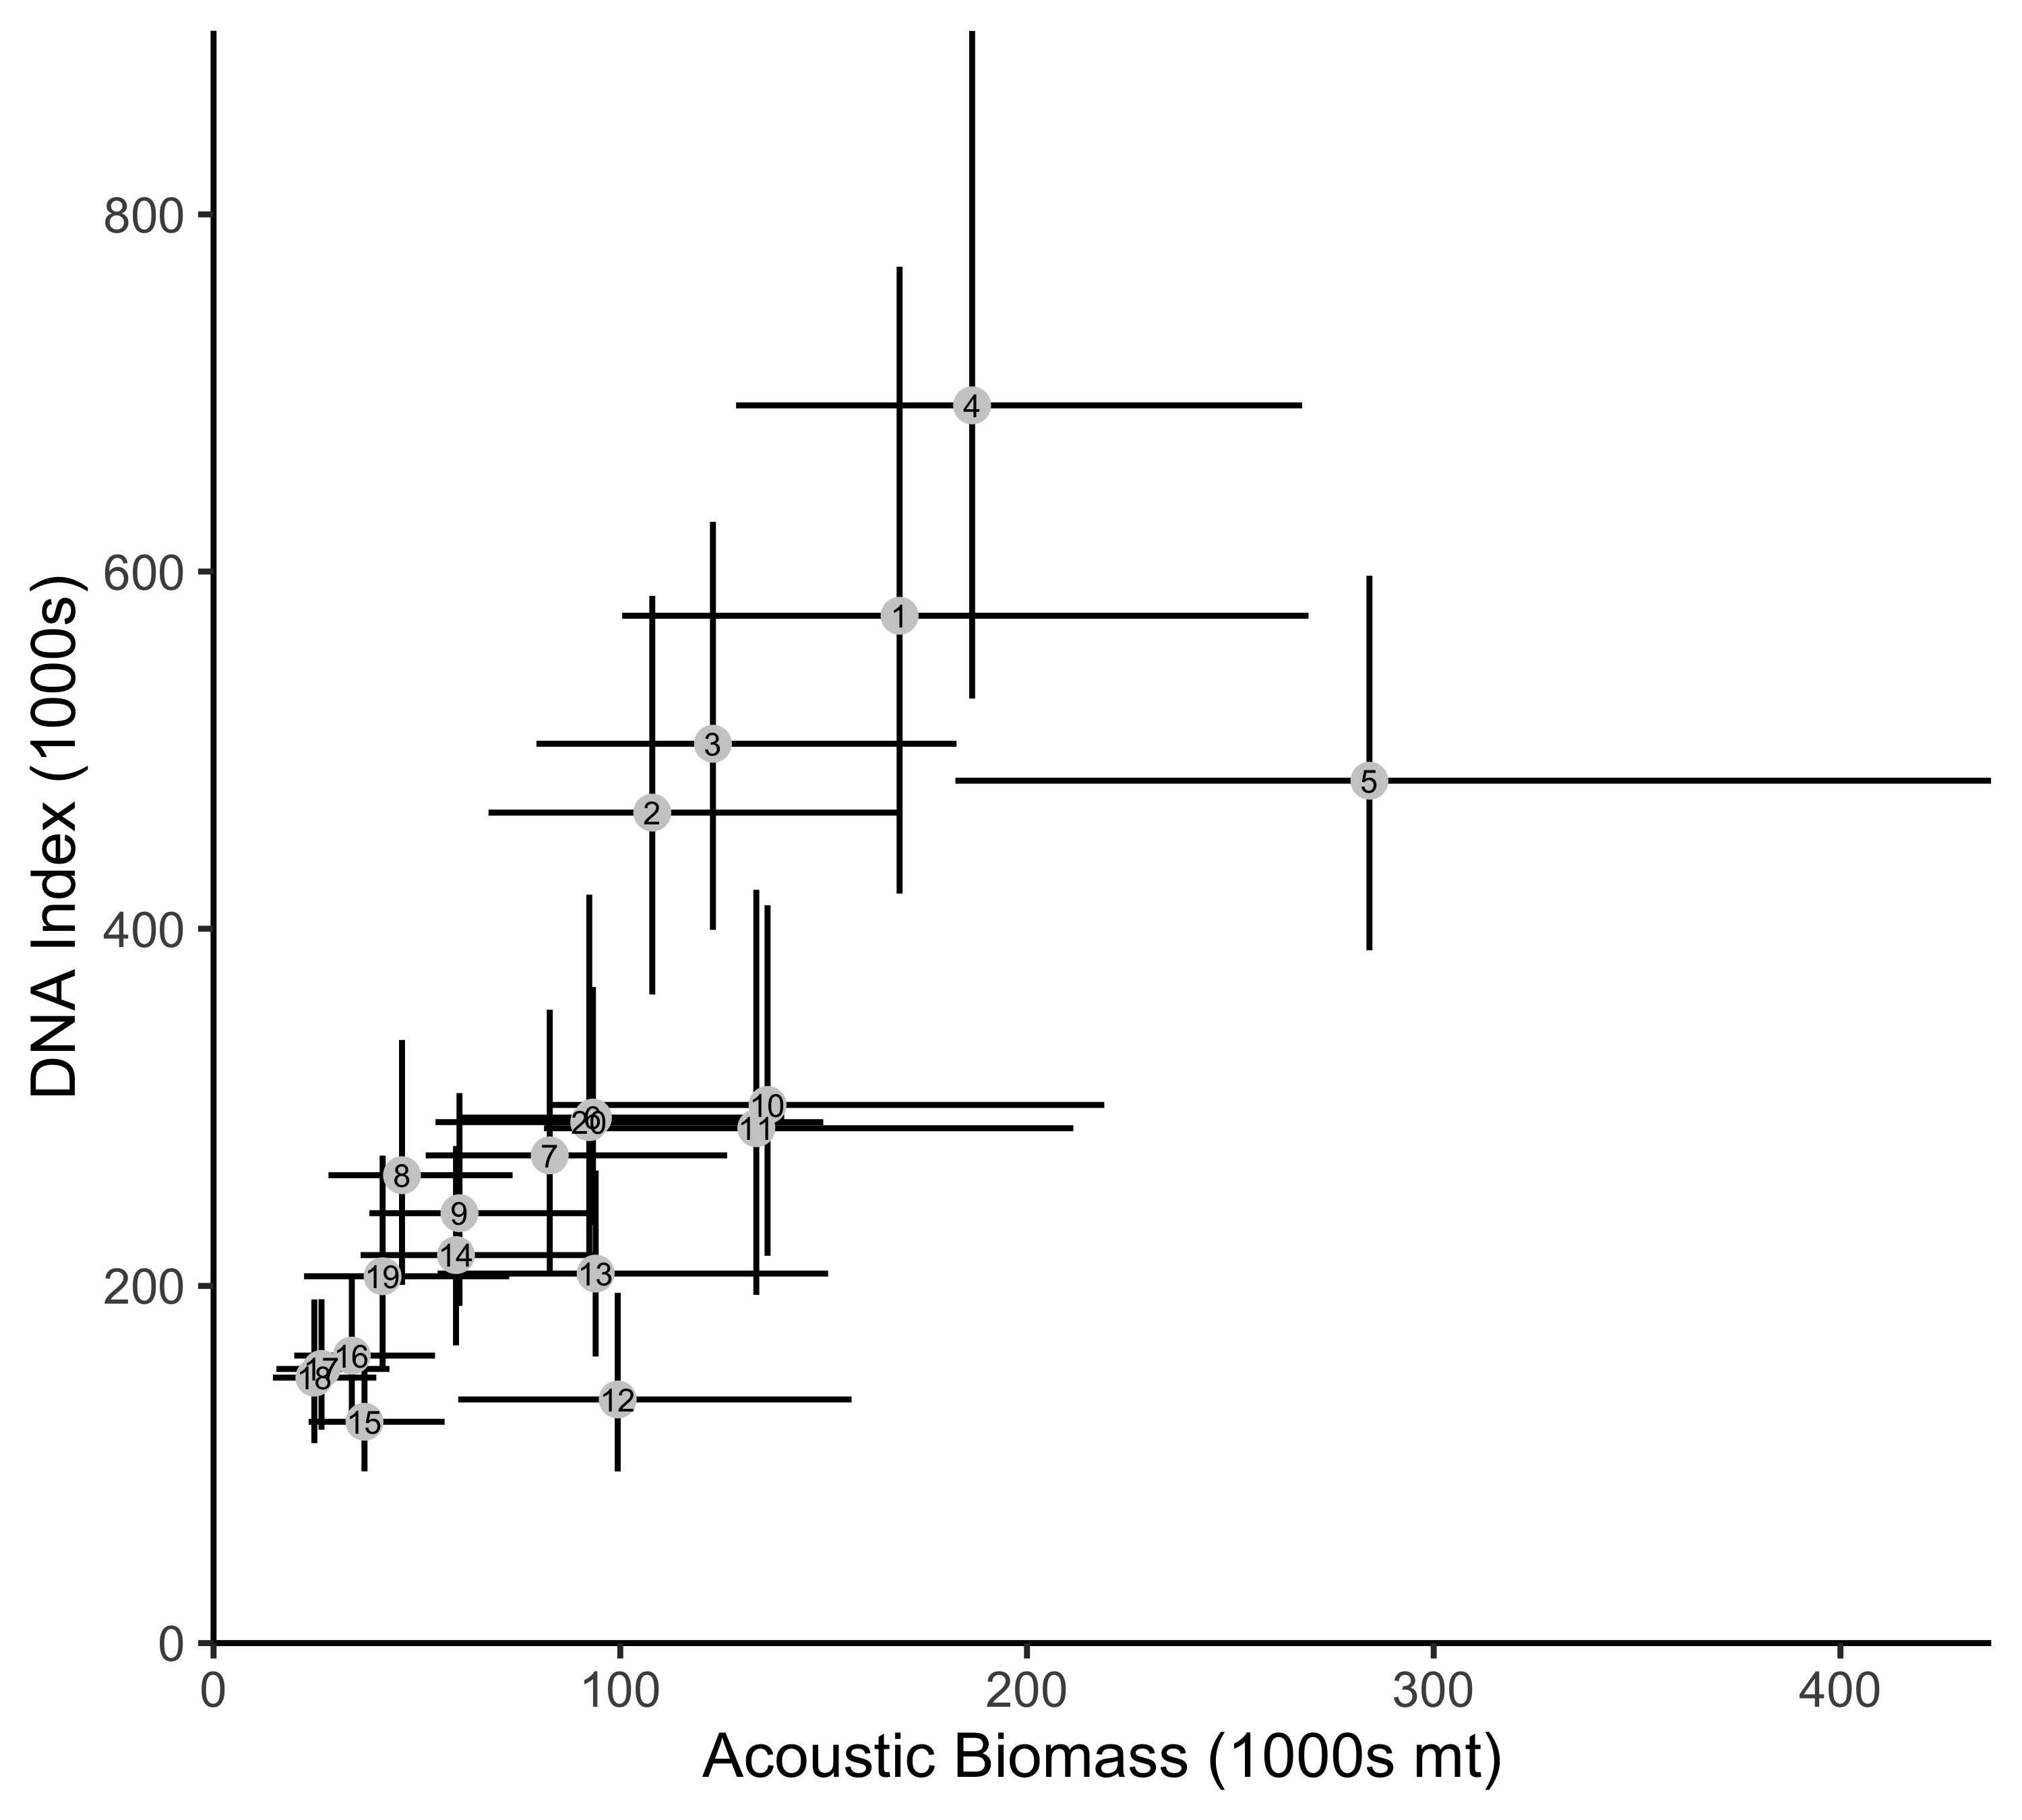
\includegraphics[width=0.6\linewidth]{./Pub_Figs/Hake_DNA-Acoustic_bivariate_correlation_0.5} \caption{\label{fig:pairwise} Pairwise comparison between  DNA and acoustics-derived biomass. Correlation between methods among the 20, half degree latitudinal bins (posterior mean, 90\% CI; \(\rho\) = 0.78{[}0.51,0.91{]}). Numbers indicate associated region identified in Fig. 2.  }\label{fig:fig.pairwise}
\end{figure}

\newpage
\clearpage

\hypertarget{acoustic-trawl-model-fit-diagnostics-and-supplementary-figures}{%
\section{Acoustic-trawl model: fit, diagnostics, and supplementary
figures}\label{acoustic-trawl-model-fit-diagnostics-and-supplementary-figures}}

The acoustic-trawl data are a depth-integrated estimate of hake density
(\(mt\) \(km^{-2}\)) along each transect line. We present the data
included in our model separated into two parts -- the occurrence or
absence of detectable hake and the hake density given occurrence (Fig.
\ref{fig:acoustic.data.maps}). See the section on the eDNA model (see
above) for description of the parameterization of smooth terms.

During prelimiary model fits, we investigated a range of knot densities
used to describe smooth terms. To balance computational speed and model
flexibility, we settled on using 5 knots for the bottom depth smooth and
a 6 (longitudinal axis) by 14 (latitudinal axis) knot grid for the
tensor-smoothes. Model results are largely insensitive to knot density.

Prior distributions for the acoustic-trawl model are presented in Table
S2.

\begin{longtable}[]{@{}ll@{}}
\caption{Prior and parameter descriptions for the Acoustic-trawl
model.}\tabularnewline
\toprule
\begin{minipage}[b]{0.47\columnwidth}\raggedright
Parameter \& Prior\strut
\end{minipage} & \begin{minipage}[b]{0.47\columnwidth}\raggedright
Description\strut
\end{minipage}\tabularnewline
\midrule
\endfirsthead
\toprule
\begin{minipage}[b]{0.47\columnwidth}\raggedright
Parameter \& Prior\strut
\end{minipage} & \begin{minipage}[b]{0.47\columnwidth}\raggedright
Description\strut
\end{minipage}\tabularnewline
\midrule
\endhead
\begin{minipage}[t]{0.47\columnwidth}\raggedright
\(\zeta_H \sim Normal(0,3)\)\strut
\end{minipage} & \begin{minipage}[t]{0.47\columnwidth}\raggedright
Spatial intercept for DNA concentration for occurrence component
\(H\)\strut
\end{minipage}\tabularnewline
\begin{minipage}[t]{0.47\columnwidth}\raggedright
\(\zeta_F \sim Normal(-1,3)\)\strut
\end{minipage} & \begin{minipage}[t]{0.47\columnwidth}\raggedright
Spatial intercept for DNA concentration for positive component
\(F\)\strut
\end{minipage}\tabularnewline
\begin{minipage}[t]{0.47\columnwidth}\raggedright
\(b_s \sim Normal(0,5)\)\strut
\end{minipage} & \begin{minipage}[t]{0.47\columnwidth}\raggedright
Linear component for each spline and tensor smooth (both \(H\) and \(F\)
model components)\strut
\end{minipage}\tabularnewline
\begin{minipage}[t]{0.47\columnwidth}\raggedright
\(s_k \sim Normal(0,\xi_k)\)\strut
\end{minipage} & \begin{minipage}[t]{0.47\columnwidth}\raggedright
Value for spline knot \(k\)\strut
\end{minipage}\tabularnewline
\begin{minipage}[t]{0.47\columnwidth}\raggedright
\(\xi_k \sim T(3,0,2.5)\)\strut
\end{minipage} & \begin{minipage}[t]{0.47\columnwidth}\raggedright
Standard deviation for spline knot \(k\)\strut
\end{minipage}\tabularnewline
\begin{minipage}[t]{0.47\columnwidth}\raggedright
\(\kappa \sim Half-Normal(0,1)\)\strut
\end{minipage} & \begin{minipage}[t]{0.47\columnwidth}\raggedright
PCR amplification standards standard deviation\strut
\end{minipage}\tabularnewline
\bottomrule
\end{longtable}

\begin{figure}
\includegraphics[width=1.05\linewidth,height=1.05\textheight]{Supplement_S1_files/figure-latex/fig.acoustic.data.maps -1} \caption{\label{fig:acoustic.data.maps} Observations from the acoustic-trawl survey of Pacific hake. Left: The occurrence (1) or absence (0) of hake biomass from each 0.926 km (0.5 nm) transect bin. Right: The biomass density observed at each positive transect bin.}\label{fig:fig.acoustic.data.maps }
\end{figure}

\hypertarget{posterior-estimates-from-the-acoustic-trawl}{%
\subsubsection{Posterior estimates from the
acoustic-trawl}\label{posterior-estimates-from-the-acoustic-trawl}}

Given the data presented in Fig. (\ref{fig:acoustic.data.maps}), we
estimate all model parameters including the smooth function of bottom
depth for each model component (Fig. \ref{fig:depth.smooth.AT}). These
marginal smooths can be compared with similar plots provided for eDNA
(see Fig. \ref{fig:depth.smooth.edna}).

\begin{figure}
\includegraphics[width=0.75\linewidth,height=1.5\textheight]{Supplement_S1_files/figure-latex/fig.depth.smooth.AT -1} \caption{\label{fig:depth.smooth.AT} Estimated marignal smooth from the spatial acoustic-trawl model for occurrence (left) and positive (right) model components. Units of the occurrence model are emph{logit} and for the positive model are \(log_e\) hake \emph{mt} \(km^{-2}\). Posterior mean and 95\% CI shown.}\label{fig:fig.depth.smooth.AT }
\end{figure}

We also generate a predictive surface for both the occurrence and
positive model using all parameter estimates (Fig.
\ref{fig:acoustic.pred.maps}). The unconditional prediction for hake
biomass concentration which combines the results from Fig.
\ref{fig:acoustic.pred.maps} is presented in Fig. 2 in the main text and
Fig. \ref{fig:surface.compare.half}.

\begin{figure}
\includegraphics[width=1.05\linewidth,height=1.05\textheight]{Supplement_S1_files/figure-latex/fig.acoustic.pred.maps-1} \caption{\label{fig:acoustic.pred.maps} Predicted surface for the probability of occurrence model (left) and conditional positive model (right; posterior predictive means shown). The unconditional mean prediction is presented in the main text (Fig. 2). }\label{fig:fig.acoustic.pred.maps}
\end{figure}

Unlike the eDNA model, there is only one parameter that controls the
variability in observed hake biomass density. As there are no replicate
observations for individual transect segments, the parameter \(\kappa\)
contains both the uncertainty about the true density in the segment
(also know as process error or process variability) and any measurement
uncertainty for a segment (the observation error or observation
variability; Fig. \ref{fig:AT.kappa}). We estimate a large value of
\(\kappa\) (\(1.46\){[}\(1.41, 1.51\){]}; posterior mean {[}95\%CI{]})
indicating large uncertainty in hake biomass density in each segment.
This uncertainty can be seen when we plot the predictions against the
observed values for both the occurrence and positive model components
(Fig. \ref{fig:AT.pred.obs})

\begin{figure}
\includegraphics[width=0.5\linewidth,height=0.5\textheight]{./Pub_Figs/Acoustics_kappa_plot_lat.long.smooth_Base_Var_6_14_6_10_smooth_hurdle} \caption{\label{fig:AT.kappa} Estimates of \(\sigma\) (\(log_e\) standard deviation hake \emph{mt} \(km^{-2}\)) for each sampling depth (posterior mean and 90\% CI shown)}\label{fig:fig.AT.kappa}
\end{figure}

\begin{figure}
\includegraphics[width=0.75\linewidth,height=1.5\textheight]{Supplement_S1_files/figure-latex/fig.AT.pred.obs -1} \caption{\label{fig:AT.pred.obs} Predicted versus observed plots for both components of the acoustic-trawl model}\label{fig:fig.AT.pred.obs }
\end{figure}

\newpage
\clearpage

\hypertarget{coordinate-reference-system}{%
\section{Coordinate reference
system}\label{coordinate-reference-system}}

The 5 km vector grid had a custom Lambert Azimuthal Equal Area
coordinate reference system - appropriate for roughly ``square'' regions
located away from the equator {]}(5){]} - that simultaneously conserved
distance and area calculations across the study region. The proj4 string
for the coordinate reference system was:

\begin{verbatim}
+proj=laea +lat_0=30.5 +lon_0=-122.6 +x_0=1000000 +y_0=0 +datum=WGS84 +units=m +no_defs
\end{verbatim}

\hypertarget{r-script-for-calculating-awm-depth}{%
\section{R script for calculating AWM
depth}\label{r-script-for-calculating-awm-depth}}

\begin{verbatim}

# calculate "weighted mean" (WM) depth value for each 5km grid cell (Fivekm_g_full),
# using value (raster) attribute table (VAT) from composite NGDC depth grid (Comp_bath_0)
# depth values are in decimeters (dm) so need to divide WM depth by 10 to convert to meters
# general equation for calculating WM for each Fivekm_g_full grid cell is:
# sum-product(depths vector and grid cell counts vector)/total grid cell count/10
# depths = Comp_bath_0 (in dm)
# grid cell counts = Count
# 5km grid cell ID# = Fivekm_g_full

# required packages
library(tidyverse)
library(magrittr)

# load .csv text file of VAT. Column types are integer, integer, integer, integer
grid_5km_raw <- read_csv("5km_grid_combined_with_ngdc_dm_FULL_vat.csv",col_types='iiii')

# calculate weighted mean for each grid cell and divide by 10 to convert depth
# from decimeters to meters
weighted_mean <- grid_5km_raw %>%
  group_by(Fivekm_g_full) %>% 
  mutate(bath_output = weighted.mean(Comp_bath_0, Count)/10)

# remove duplicate rows in weighted_mean
dupe_remove <- weighted_mean[!duplicated(weighted_mean[ , c("Fivekm_g_full","bath_output")]),]

# create df with renamed 5km grid cell ID and weighted mean columns
dupe.sub <- dupe_remove %>% select(Fivekm_g_full, bath_output) %>%
  set_colnames(c("Gridcell_ID", "wm_ngdc_depth_m"))
\end{verbatim}

\clearpage

\hypertarget{citations}{%
\section*{Citations}\label{citations}}
\addcontentsline{toc}{section}{Citations}

\hypertarget{refs}{}
\leavevmode\hypertarget{ref-deBlois2020survey}{}%
1. S. de Blois, The 2019 joint U.S.--Canada integrated ecosystem and
Pacific hake acoustic-trawl survey: Cruise report sh-19-06. \emph{U.S.
Department of Commerce, NOAA Processed Report NMFS-NWFSC-PR-2020-03}
(2020).

\leavevmode\hypertarget{ref-ramon-laca2021PLOS}{}%
2. A. Ramón-Laca, A. Wells, L. Park, A workflow for the relative
quantification of multiple fish species from oceanic water samples using
environmental dna (eDNA) to support large-scale 2021. \emph{PLoS ONE}
\textbf{16}, e0257773 (2021).

\leavevmode\hypertarget{ref-brms2017}{}%
3. P.-C. Bürkner, brms: An R package for Bayesian multilevel models
using Stan. \emph{Journal of Statistical Software} \textbf{80}, 1--28
(2017).

\leavevmode\hypertarget{ref-brms2018}{}%
4. P.-C. Bürkner, Advanced Bayesian multilevel modeling with the R
package brms. \emph{The R Journal} \textbf{10}, 395--411 (2018).

\leavevmode\hypertarget{ref-snyder1987map}{}%
5. J. P. Snyder, \emph{Map projections--a working manual} (US Government
Printing Office, 1987).

\end{document}
